\chapter{Côté Serveur}


\section{Structuration du code}

Pour notre architecture nous avons structuré le code en trois parties : le client, la configuration et le serveur.

\begin{itemize}
    \item \textbf{Client} : Il gère la communication avec le serveur. Il a aussi son propre \textit{main}.
    \item \textbf{Configuration} : Il contient la classe \textit{Config.java} et le fichier \textit{config.json} pour la configuration des paramètres de l'application. Ce sont les bonnes pratiques de sécurité qui nous ont poussés à faire ceci.
    \item \textbf{Serveur} : Il comprend différents sous-modules :
    \begin{itemize}
        \item \textbf{Base de données} : Ce module gère la connexion à la base de données ainsi que les opérations sur cette dernière.
        \item \textbf{Éléments} : Défini les entités de l’application telles qu’un \textit{Document} et un \textit{Abonne}.
        \item \textbf{Exceptions} : Gère les différentes exceptions spécifiques à l’application.
        \item \textbf{Opérations} : Regroupe les différents services de l’application (Réservation, Emprunt, Retour).
        \item \textbf{Serveur} : Implémente le protocole de communication utilisé par l’application.
        \item \textbf{Utilitaire} : Fournit des méthodes utiles à l’application et donc réutilisables.
        \item \textbf{TimerTask} : Ce module permet de gérer les tâches planifiées.
    \end{itemize}
    Le serveur a aussi son propre \textit{main} afin d'être exécuté indépendamment du client.
\end{itemize}


\section{Code Stable}

Pour ce projet, nous avons mis en place plusieurs dispositifs pour rendre le code maintenable et stable.

Premièrement, nous avons utilisé des \textcolor{red}{factories} pour faciliter la création d'éléments en grande quantité. Nous avons implémenté une factory dédiée aux serveurs ce qui nous permet de générer autant de serveurs que nécessaire. Cela nous offre la flexibilité de remplacer ou mettre à jour un serveur sans affecter le reste du code.

Une factory pour les données a été mise en place pour charger les données depuis la base de données lors de l’initialisation de l’application et de les sauvegarder lors de la fermeture de l’application. Ces factories évitent la répétition de tâches redondantes et utilisent les classes de modèle ou de serveur comme objets, conformément aux notions étudiées en cours. Cela rend les factories plus \textcolor{blue}{évolutives et adaptables}.

Nous avons également mis en place des interfaces pour assurer la stabilité des classes. De plus, pour certaines parties du code, nous avons factorisé les méthodes et les variables en les regroupant dans une seule classe, permettant ainsi aux autres classes d’hériter de celle-ci.

L’objectif est de faire en sorte que nos classes respectent au mieux les principes \textcolor{blue}{SOLID} et les design patterns vus en cours de qualité logicielle, tels que le pattern Factory, le pattern Bridge et autres patterns de conception. Cela permet d'assurer une architecture de code robuste, flexible et facile à maintenir.


\section{Graphe de dépendance}

\begin{figure}[H]
    \centering
    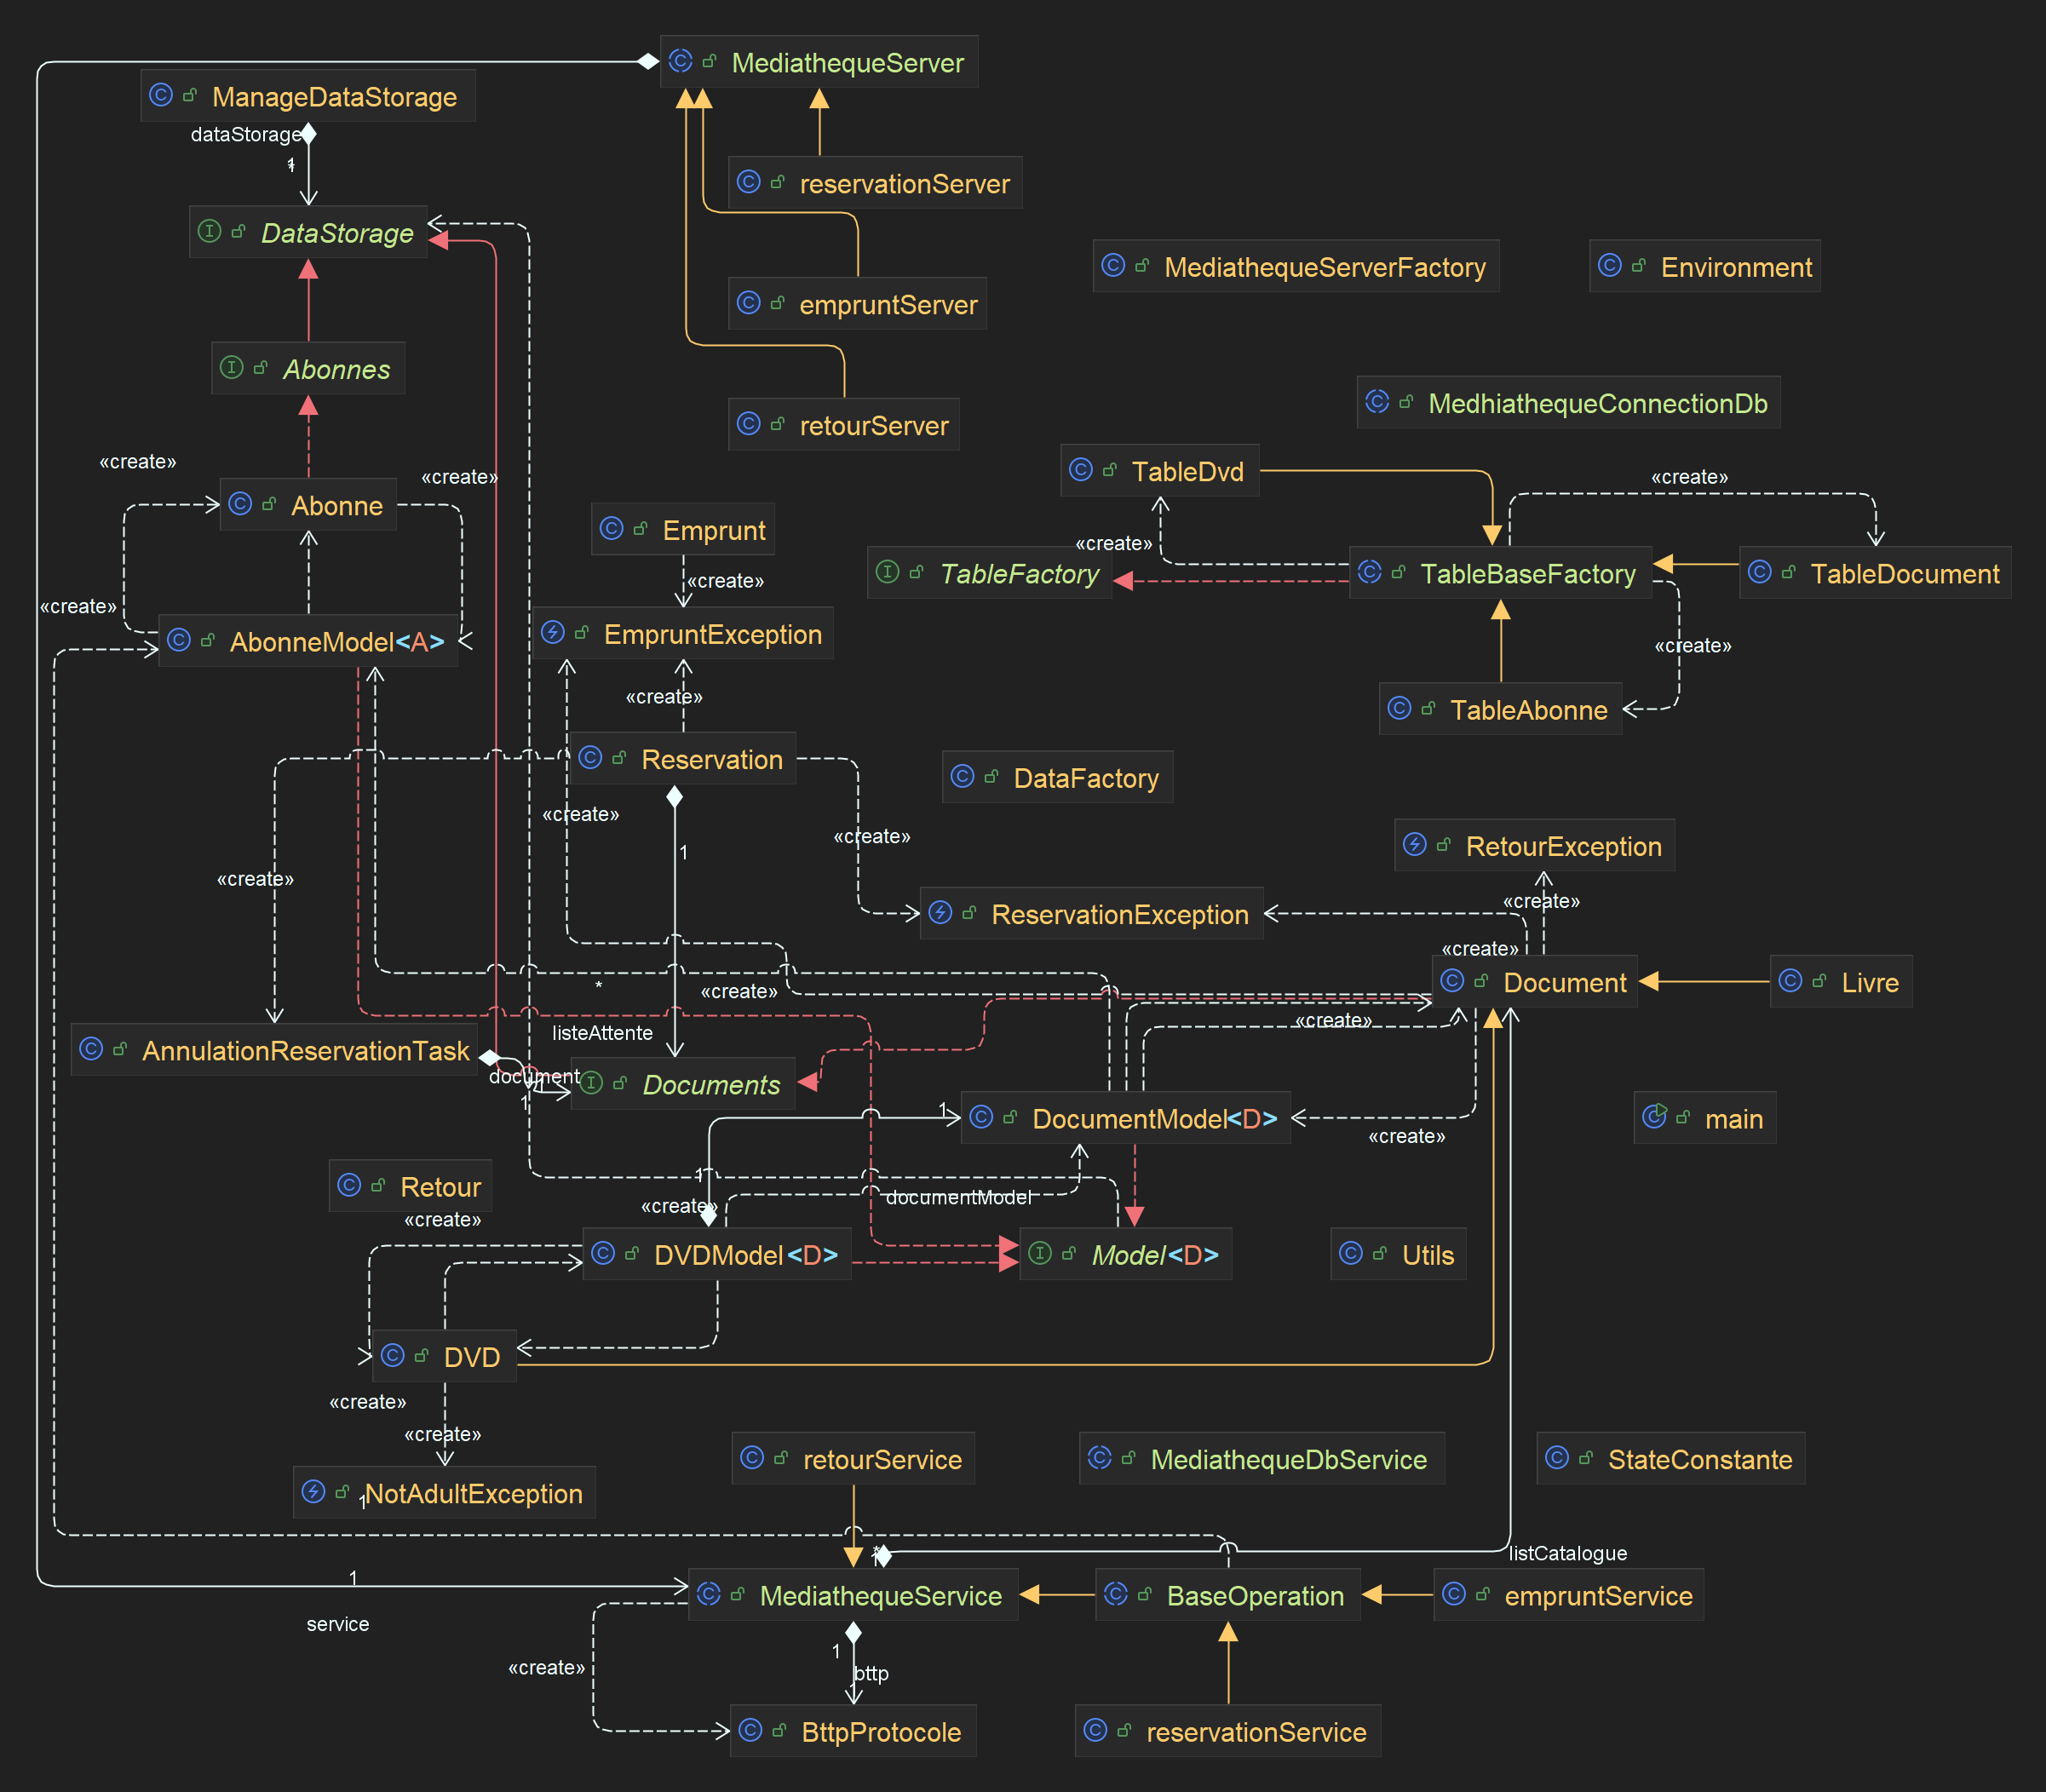
\includegraphics[width=1.1\textwidth]{image/uml5}
    \caption{Graphe de dépendance}
    \label{fig:dependency_graph}
\end{figure}


\section{Bibliothèques logicielles}

Nous avons utilisé plusieurs bibliothèques logicielles essentielles pour développer le projet. Voici les bibliothèques utilisées et leur utilisation spécifique :

\begin{itemize}
    \item \textbf{JDBC} : Cette bibliothèque a été utilisée pour interagir avec la base de données, permettant d'exécuter des requêtes SQL et de gérer les connexions conformément aux principes vus en cours.
    \item \textbf{Java .net} : Elle a été employée pour créer un protocole de communication via \textit{ServerSocket}, facilitant les échanges entre le client et le serveur.
    \item \textbf{Java .io} : Nous avons utilisé cette bibliothèque pour gérer les opérations d'entrée et de sortie, telles que la lecture et l'écriture de données ainsi que les exceptions associées.
    \item \textbf{Org .json} : Cette bibliothèque a été utilisée pour lire et traiter le fichier \textit{config.json}, ce qui nous permet de gérer les paramètres de configuration de manière sécurisée et flexible.
    \item \textbf{Java .util} : Nous avons largement utilisé cette bibliothèque pour manipuler différentes collections (\textit{Map}, \textit{List}), ainsi que pour les fonctionnalités de \textit{Scanner}, \textit{Date}, \textit{Timer} et \textit{TimerTask}. \textit{TimerTask} a été implémenté afin de limiter la durée maximale d'une réservation pour emprunter un document, évitant ainsi des réservations indéfinies.
    \item \textbf{Java .sql} : Cette bibliothèque a été intégrée pour permettre la communication en SQL avec la base de données, facilitant ainsi les opérations de création, lecture, mise à jour et suppression (CRUD) en utilisant également les exceptions spécifiques de cette bibliothèque.
\end{itemize}

L'utilisation de ces bibliothèques a permis de structurer notre application de manière efficace, en utilisant des outils et fonctionnalités standards de Java pour assurer maintenabilité et performance.
